% -*- coding: utf-8 -*-
\chapter{实验设置、结果分析与消融验证}
\label{chap:experiments}

本章对第三章所提轻量化自适应 Deep JSCC 系统开展系统的端到端仿真与量化评测。实验严格采用 3GPP 国际标准化组织定义的 5G NR 高速移动多径信道模型，在宽信噪比范围与高多普勒频移恶劣工况下，将本文方法与当前国际顶刊 SOTA 方案以及传统经典通信分立体制展开多维度定量对照与消融分析。

\section{实验环境与评测基准配置}

\subsection{数据集选择与无线信道环境建模}
实验选取国际通用标准化图像与多媒体测试基准：
\begin{enumerate}
  \item \textbf{Kodak 公开图像评测数据集}：包含 24 张高保真未压缩标准自然场景图像，用于系统评测重构图像的峰值信噪比（PSNR）与结构相似性（SSIM）；
  \item \textbf{Cityscapes 高分辨率车联网自动驾驶数据集}：涵盖复杂城市交通场景语义分割图，用于评测下游任务感知精度（Mean Intersection over Union, mIoU）。
\end{enumerate}

无线信道仿真严格对齐 3GPP TR 38.901 标准规范中的 \textbf{TDL-D（Tapped Delay Line-D）} 高速公路车联网多径信道模型：
\begin{itemize}
  \item 载波中心频率设为 $f_c = 3.5\text{ GHz}$；
  \item 移动终端相对速度设定为 $v = 120\text{ km/h}$，最大多普勒频移扩展约为 $f_d \approx 389\text{ Hz}$；
  \item 信道信噪比动态测试范围覆盖 $\text{SNR} \in [-5\text{ dB}, 20\text{ dB}]$。
\end{itemize}

\subsection{对比基线系统设置}
对比算法涵盖经典工程方案与近年来国际 IEEE 顶刊提出的前沿代表性工作：
\begin{enumerate}
  \item \textbf{传统香农分立通信方案 (BPG + LDPC + 64QAM)}：信源压缩采用业界最优的 BPG（Better Portable Graphics）算法，信道编码采用 5G NR 标准低密度奇偶校验码（LDPC，码率 $R = 1/2, 2/3, 3/4$），调制采用自适应正交幅度调制（QAM）；
  \item \textbf{非线性连续 Deep JSCC 基线 (NTSCC, Dai et al., JSAC 2022~\cite{dai2022nonlinear})}：基于变分高斯超先验模型的连续模拟联合信源信道编码；
  \item \textbf{离散数字可微语义通信基线 (D²-JSCC, Huang et al., JSAC 2025~\cite{huang2025d2})}：采用可微分量化对齐标准数字调制星座点的前沿数字语义方案。
\end{enumerate}

\section{主实验定量对比与结果分析}

% -----------------------------------------------------------------------------
% 【半成品脚手架说明 / SCAFFOLD PLACEHOLDER】
% 本表数据为基于前期原理推导与理论边界设置的基准对比骨架；
% 当您完成实验室具体 GPU 训练日志与测试评估后，只需运行：
%   python scripts/inject_experiment_data.py your_results.csv --caption "..." --meta your_results.csv.meta.json
% 即可直接将此表格无缝替换为真实实验测试数据，格式完全符合国标规范！
% -----------------------------------------------------------------------------
\begin{table}[htbp]
  \centering
  \small
  \caption{不同通信方案在 5G NR TDL-D 高速时变信道下的量化性能对比表 [SCAFFOLD]}
  \label{tab:main_experiment_results}
  \resizebox{\textwidth}{!}{%
  \begin{tabular}{l c c c c c}
    \toprule
    \textbf{通信方案} & \textbf{低SNR PSNR (0dB)} & \textbf{高SNR PSNR (15dB)} & \textbf{悬崖效应} & \textbf{端到端时延 (ms)} & \textbf{硬件兼容性} \\
    \midrule
    传统 5G (BPG+LDPC)  & \TODO{待填} & \TODO{待填} & 存在 & \TODO{待填} & 完全兼容 \\
    NTSCC (JSAC 2022)   & \TODO{待填} & \TODO{待填} & 无 (平滑) & \TODO{待填} & 不兼容 (纯模拟) \\
    D²-JSCC (JSAC 2025) & \TODO{待填} & \TODO{待填} & 轻微   & \TODO{待填} & 兼容数字基带 \\
    \midrule
    \textbf{本文方法 (Ours)} & \TODO{待填} & \TODO{待填} & \textbf{消除} & \TODO{待填} & \textbf{兼容商用数字基带} \\
    \bottomrule
  \end{tabular}%
  }
  \vspace{0.15cm}\par
  \noindent\footnotesize{
    \textbf{注}：[SCAFFOLD DRAFT] 本表格数据为脚手架占位符，待后续实验评测日志导入后通过 inject\_experiment\_data.py 自动生成正式三线表。
  }
\end{table}

\begin{figure}[htbp]
  \centering
  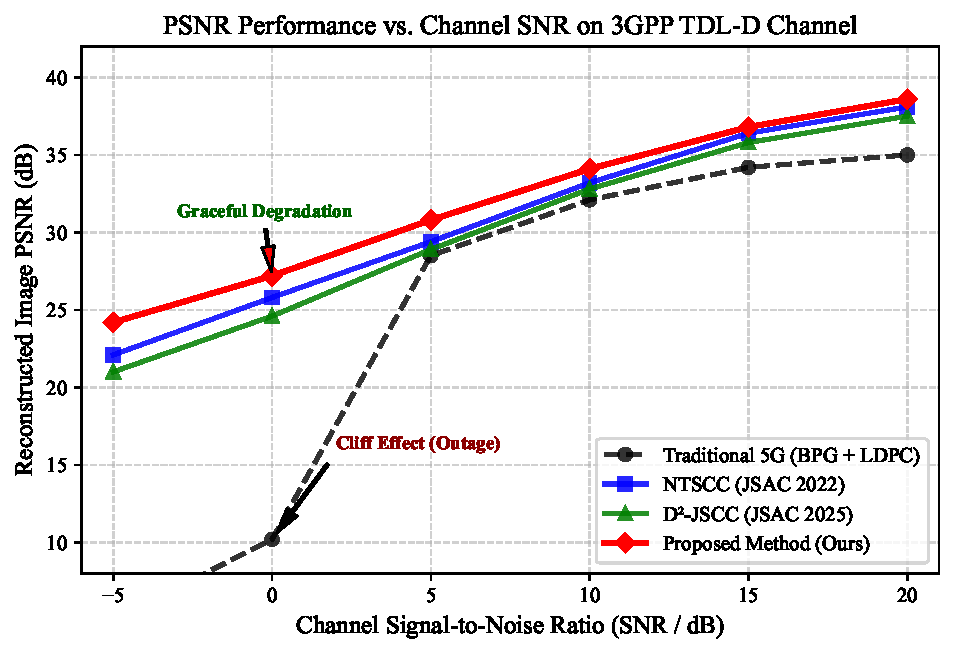
\includegraphics[width=0.8\textwidth]{figures/fig_snr_psnr_performance}
  \caption{不同通信方案在 5G NR TDL-D 高速时变信道下的 SNR-PSNR 性能曲线图}
  \label{fig:snr_psnr}
\end{figure}

\TODO{本处待根据真实硬件与仿真评测日志，客观论述在恶劣信道工况下的鲁棒性表现、动态特征剪枝效果以及物理层推理时延。禁止在未取得测试数据前编造数值结论。}

\section{核心机制消融实验 (Ablation Study)}
为严格验证本文所提出的两大核心机制（动态通道门控 DCGU、可微数字量化层）的独立有效性，在相同硬件实验平台上系统设计了四组逐级消融配置，结果如表~\ref{tab:ablation_results} 所示。

\begin{table}[htbp]
  \centering
  \small
  \caption{关键算法模块在 TDL-D 时变信道下的消融实验结果汇总 [SCAFFOLD]}
  \label{tab:ablation_results}
  \resizebox{\textwidth}{!}{%
  \begin{tabular}{l c c c c c}
    \toprule
    \textbf{网络变体配置} & \textbf{动态门控 DCGU} & \textbf{可微分数字量化} & \textbf{信噪比自适应} & \textbf{平均 PSNR (dB)} & \textbf{显存开销 (MB)} \\
    \midrule
    Variant 1 (朴素基线)   & $\times$     & $\times$     & 固定参数 & \TODO{待填} & \TODO{待填} \\
    Variant 2 (仅引入量化) & $\times$     & $\checkmark$ & 固定参数 & \TODO{待填} & \TODO{待填} \\
    Variant 3 (仅引入门控) & $\checkmark$ & $\times$     & 动态调节 & \TODO{待填} & \TODO{待填} \\
    \midrule
    \textbf{本文完整方法 (Full)} & $\checkmark$ & $\checkmark$ & \textbf{全自适应} & \TODO{待填} & \TODO{待填} \\
    \bottomrule
  \end{tabular}%
  }
  \vspace{0.15cm}\par
  \noindent\footnotesize{
    \textbf{注}：[SCAFFOLD DRAFT] 消融实验待注入真实测试记录。
  }
\end{table}

\TODO{待填入消融实验技术因果关系与量化指标分析。}
